\chapter{Algebra 3}
\section{Sequences}
When we have a list of numbers that follow a pattern this is called a sequence.  Patterns in mathematics are very important and we are typically interested in how they are created and how they look when they are plotted on a graph.  In this chapter we will mainly be looking at sequences that produce straight lines when we draw them, these are called linear sequences.
\subsection{Generating a Sequence}
We learnt in the first chapter how to substitute values into a formula, that is what we are going to do here.

Consider the equation $n^{th}=4n+7$.  To find the $1^{st}$ term we just let $n=1$, to find the $2^{nd}$ term we just let $n=2$ and so on.

\bigskip

\begin{exmp}
Let's find the first five terms for the sequence generated by the formula $n^{th}=4n+7$

\bigskip

Let $n=1$ therefore the first term is $4 \times 1 + 7 = 11$

\bigskip

Let $n=2$ therefore the first term is $4 \times 2 + 7 = 15$

\bigskip

Let $n=3$ therefore the first term is $4 \times 3 + 7 = 19$

\bigskip

Let $n=4$ therefore the first term is $4 \times 4 + 7 = 23$

\bigskip

Let $n=5$ therefore the first term is $4 \times 5 + 7 = 27$

\bigskip

The first five terms are 11, 15, 19, 23, 27.

\end{exmp}

\begin{exmp}
Find the $25^{th}$ term of the sequence with the formula $n^{th} = 3n-10$

\bigskip

Let n = 25

\bigskip

So $25^{th} = 3 \times 25 - 10 = 65$
\end{exmp}

\subsection{Exercise}
Find the first 10 terms of the following sequences:
\begin{enumerate}
	\item $n^{th}=2n+14$
	\item $n^{th}=5n-4$
	\item $n^{th}=8n+2$
	\item $n^{th}=2n-1$
	\item $n^{th}=3n+2$
	\item $n^{th}=-3n+20$
	\item $n^{th}=6n$
	\item $n^{th}=n^2$
	\item $n^{th}=7n-7$
	\item $n^{th}=-n$
\end{enumerate}

\subsection{Finding a formula for a sequence}
We are now going to develop a method for finding the formula for a linear sequence when we know the sequence.

First, let's consider the first five terms of $n^{th}=5n$.  They are 5, 10, 15, 20, 25.

Now, let's consider the first five terms of $n^{th}=3n$.  They are 3, 6, 9, 12, 15.

You might notice that formula of this type produce the times tables.  Therefore if we wanted the 4 times table we would use the formula $n^{th}=4n$.


\begin{exmp}
Find the formula for the sequence: 6, 12, 18, 24, 30, ...

\bigskip

Since the sequence is just the 6 times table the formula must be $n^{th}=6n$.
\end{exmp}

\begin{exmp}
Find the formula for the sequence: -4.5, -9, -13.5, -18, -22.5, ...

\bigskip

If this were a times table it would be the -4.5 times table, since it starts at -4.5 and goes down by 4.5 each time.  Therefore the formula is $n^{th}=-4.5n$
\end{exmp}

Now let's consider the sequence 5, 8, 11, 14, 17, ... .  The sequence goes up by 3 each time like the 3 times table, so it would make sense that $3n$ is part of the formula.  However, the numbers in this sequence are all 2 more than the 3 times table so that makes the formula $n^{th}=3n+2$.

\bigskip

To find the formula for a linear sequence we first find out how much it is going up by each time and then work out what adjustment we have to make to the corresponding times table to get our sequence.

\begin{exmp}
Find the formula for the sequence: 5, 9, 13, 17, 21, ...

\bigskip

This sequence goes up by 4 each time like the 4 times table so that would imply $n^{th}=4n$, but our values are always 1 more, so the formula is $n^{th}=4n+1$.
\end{exmp}

\begin{exmp}
Find the formula for the sequence: 3, 8, 13, 18, 23 ...

\bigskip

This sequence goes up by 5 each time like the 5 times table so that would imply $n^{th}=5n$, but our values are always 2 less, so the formula is $n^{th}=5n-2$.
\end{exmp}

\begin{exmp}
Find the formula for the sequence: 10, 7, 4, 1, -2, ...

\bigskip

This sequence goes down by 3 each time like the -3 times table so that would imply $n^{th}=-3n$, but our values are always 13 more, so the formula is $n^{th}=-3n+13$.
\end{exmp}
\subsection{Exercise}
Find the formula for the following sequences:
\begin{enumerate}
	\item 3, 9, 15, 21, 27, ...
	\item 7, 9, 11, 13, 15, ...
	\item 10, 10.5, 11, 11.5, 12, ...
	\item 3, 1, -1, -3, -5, ...
	\item 0, 2, 4, 6, 8, ...
	\item 9, 10, 11, 12, 13, ...
	\item 8, 15, 22, 29, 36, ...
	\item 8, 1, -6, -13, -20, ...
	\item 8, 5.5, 3, 0.5, -2, ...
	\item 6, 6, 6, 6, 6, ...
\end{enumerate}
\subsection{Plotting a Sequence}
We can plot a sequence on a graph and if it is a linear sequence the points make a straight line.  Consider the sequence 2, 5, 8, 11, 14, ...

\bigskip

We turn these numbers into pairs of coordinates (term position, term value)

\bigskip

So here we get

\begin{itemize}
	\item $(1,2)$
	\item $(2,5)$
	\item $(3,8)$
	\item $(4,11)$
	\item $(5,14)$
\end{itemize}

If we plot these on a graph we get:

\begin{center}
	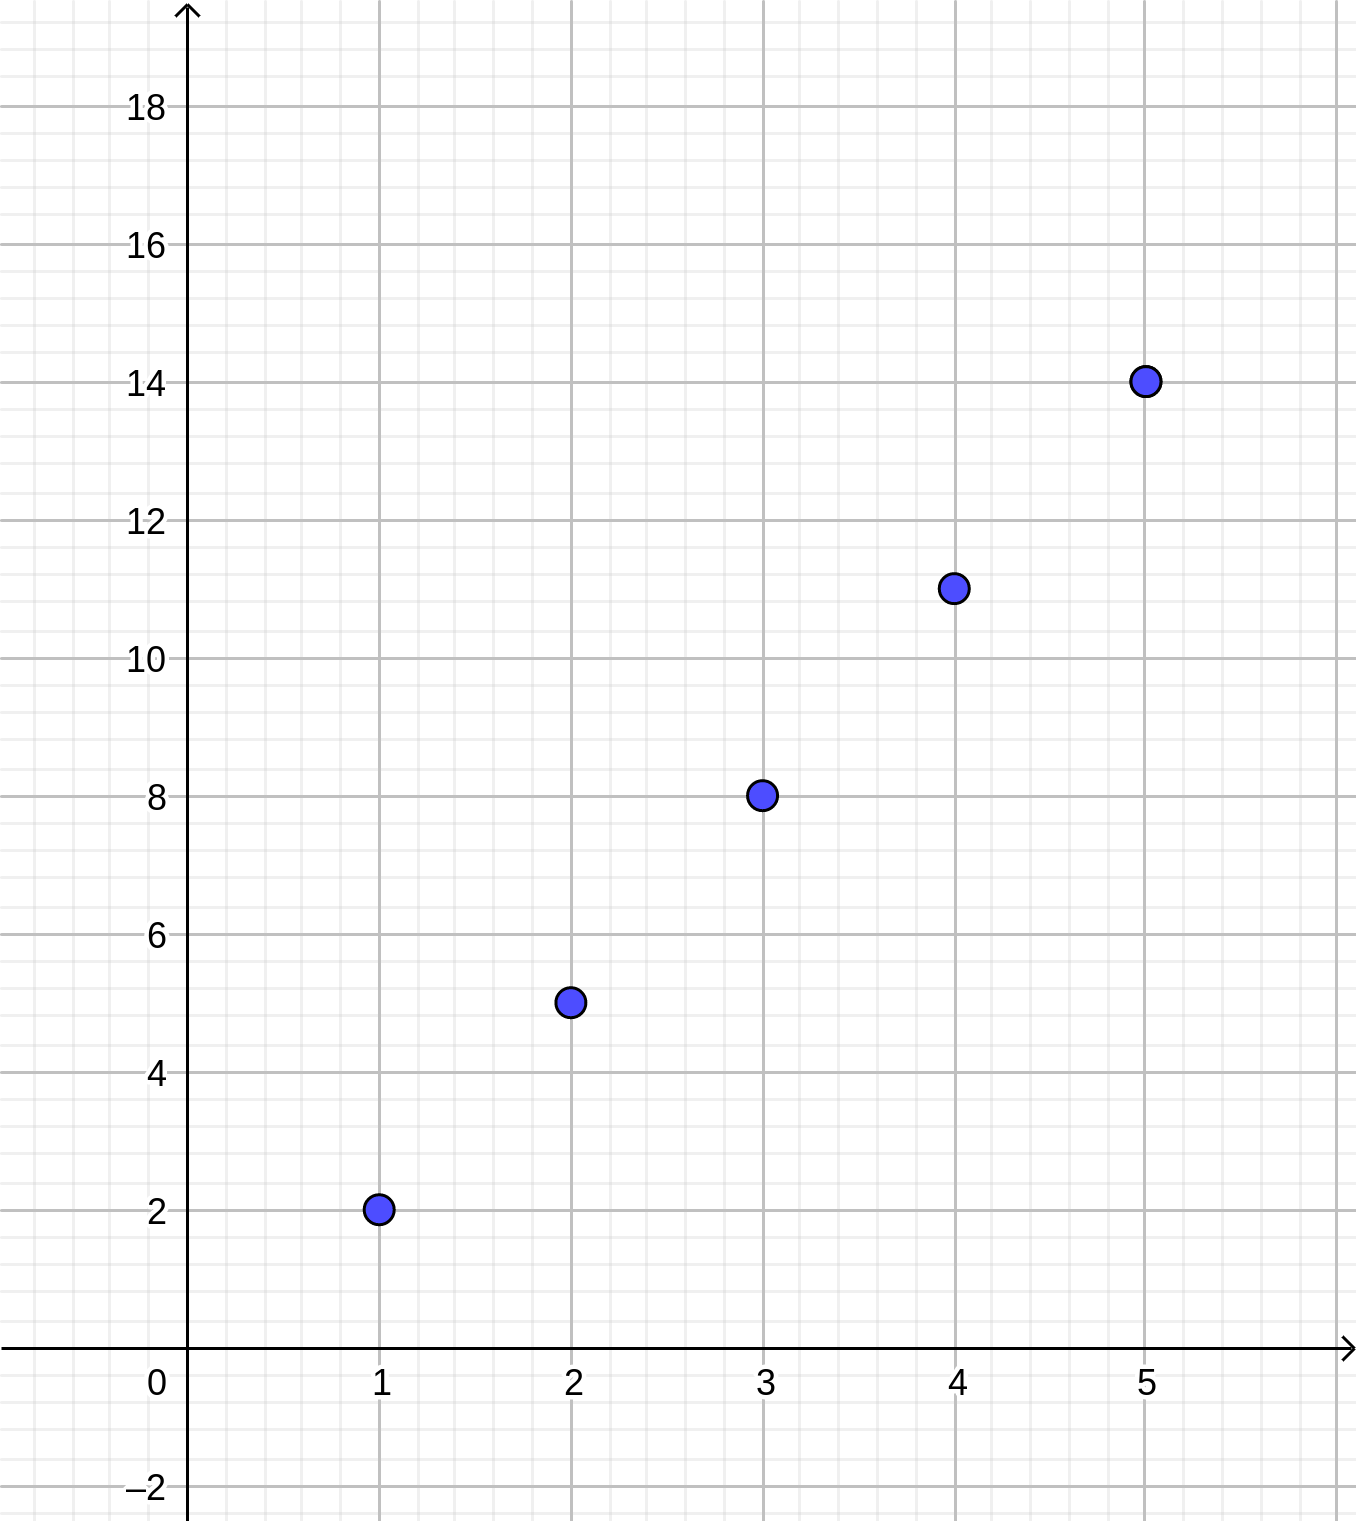
\includegraphics[height=8.4cm,keepaspectratio]{./Images/Algebra/seqPlot}
\end{center}

\subsection{Exercise}
Plot on an appropriate set of axes the points corresponding to the sequences below:
\begin{enumerate}
	\item 3, 9, 15, 21, 27, ...
	\item 7, 9, 11, 13, 15, ...
	\item 10, 10.5, 11, 11.5, 12, ...
	\item 3, 1, -1, -3, -5, ...
	\item 0, 2, 4, 6, 8, ...
	\item 9, 10, 11, 12, 13, ...
	\item 8, 15, 22, 29, 36, ...
	\item 8, 1, -6, -13, -20, ...
	\item 8, 5.5, 3, 0.5, -2, ...
	\item 6, 6, 6, 6, 6, ...
	\item $n^{th}=2n+14$
	\item $n^{th}=5n-4$
	\item $n^{th}=8n+2$
	\item $n^{th}=2n-1$
	\item $n^{th}=3n+2$
	\item $n^{th}=-3n+20$
	\item $n^{th}=6n$
	\item $n^{th}=n^2$
	\item $n^{th}=7n-7$
	\item $n^{th}=-n$
\end{enumerate}

You can see that these points make a straight line if they are connected together.
\subsection{Special Sequences}
The special sequences that we are going to look at are: odd numbers, even numbers, square numbers and triangular numbers.  We will consider the numbers in their sequence and the formulae that produce them.

\subsubsection{Odd numbers}
The odd numbers go 1, 3, 5, 7, 9, ... . We can see that this is a linear sequence so that means that we know how to create a formula for it.  It goes up by 2 each time like the 2 times table, but all these values are 1 less, that implies that the formula is $n^{th}=2n-1$

\subsubsection{Even numbers}
The even numbers go 2, 4, 6, 8, ... . We can see that this is a linear sequence so that means that we know how to create a formula for it.  It goes up by 2 each time like the 2 times table, with no change, that implies that the formula is $n^{th}=2n$

\subsubsection{Square numbers}
Square numbers are calculated by counting the number of dots required to make a square.  So for example, if a square was 4 high and 4 wide we would need a total of 16 dots (4 rows of 4), this gives us the $4^{th}$ square number.  The first 5 square numbers in order are: 1, 4, 9, 16, 25.  The formula for finding square numbers is $n^{th}=n^2$

\subsubsection{Triangular numbers}
Triangular numbers are the number of dots that we get when we count the number of dots in a triangle.  Imagine a triangle with 1 dot at the top, 2 dots on the 2nd layer, 3 dots on the 3rd layer, 4 dots on the 4th layer and so on, these are the kind of triangles we are talking about.  So the 4th triangular number would come from a triangle with 4 layers, the number of dots would be $1+2+3+4=10$.  So the 4th triangular number is 10.

\subsection{Exercise}
With the following sequences compare them to the sequence of Square numbers and see if you can work out their formula would be:
\begin{enumerate}
	\item $2,5,10,17,26,37,...$
	\item $0,3,8,15,24,35,...$
	\item $11,14,19,26,35,46,...$
	\item $2,8,18,32,50,72,...$
\end{enumerate}
With the following sequences compare them to the sequence of Triangular numbers and see if you can work out their formula would be:
\begin{enumerate}
	\item $6,8,11,15,20,...$
	\item $0,2,5,9,14,...$
	\item $8,10,13,17,22,...$
	\item $2,6,12,20,30,...$
\end{enumerate}

\subsection{Solving for a sequence}
We are going to look at situations where we know the first part of the sequence.  From this we can work out the formula and then use the formula to work out which term has a particular value.

\begin{exmp}
If we have the sequence $5, 12, 19, 26, ...$ which term has the value 96?

First we want the formula for the sequence.  Our sequence goes up by 7 each time like the 7 times table, but each term is 2 less, so our formula is $n^{th}=7n-2$.

Now we know our particular nth term has a value of 96, so let's make the equation:

$7n-2=96$

If we solve this equation we get $n=14$, so it is the 14th term which equals 96.
\end{exmp}

\subsection{Exercise}
\begin{enumerate}
	\item For the sequence $4,10,16,22,...$ which term has the value $118$?
	\item For the sequence $9,13,17,21,...$ which term has the value $209$?
	\item For the sequence $27, 25, 23, 21, ...$ which term has the value $-117$?
	\item For the sequence $19,30,41,52,...$ which term has the value $481$?
\end{enumerate}

\subsection{Sequences in other situations}
When a given situation seems to follow a pattern we can often assign this to a sequence.

\begin{exmp}
Suppose a train engine is 10 m long and carridges are 7 m long. Train design 1 has 1 carridge and train design 2 has 2 carridges etc. Which train design is 59 m long.

First let's make a sequence for the different designs:

\bigskip

$17, 24, 31, 38...$

\bigskip

We can see that the formula for this sequence is $n^{th}=7n+10$ when $n$ is the design number and $n^{th}$ represents the length of the train.

\bigskip

So the equation we need to solve is $7n+10=59$ and the result is $n=7$.  So it is design 7 which is 59 m long.
\end{exmp}
\subsection{Exercise}
\begin{enumerate}
	\item A gardener buys a tree that is 1m tall and grows at a rate of 0.2m per year.  So at the end of the first year it is 1.2m tall.  Write a formula for how tall the tree will be after year 'n' and use this formula to work out the height of the tree after 11 years.
	\item A boy got a score of 17 on a maths test and decided to put in place a study program to improve.  The study program helped him improve his score by 3 each week, so that after 1 week he would get a score of 20.  Use a formula to calculate his score after 9 weeks and calculate after how many weeks it would be for him to get a score of 80.
	\item In my Youtube account I have 3478\cent \hspace{0.2cm} and I earn 87\cent \hspace{0.2cm} a day.  After how many days will it be for me to have a total of \$507?
	\item Rose was growing a rose. The flower grew 0.3 metres each week. It is 0.8 metres right now. How long will the flower be in 52 weeks? (1 year) (R.H.)
	\item Alice plants daisies.  In the first summer she planted 50 seeds and plants 17 more seeds in the each of the following summers.  How many seeds would she have planted in the first 15 years? (K.W.)
	\item Isobel decides to sail from New Zealand to Japan, she starts counting how many Kms she has travelled per day after she knows she has travelled 12km.  The next day she sees that she has now gone 21km.  If she continues at the same speed, how far will she have travelled after 11 days.  Also how far will she have travelled after 'n' days?  If it is 9346km to Japan how long will it take her to get there. (I.F.)
\end{enumerate}
